\documentclass{standalone}

\usepackage[english]{babel}

% to define font size

\usepackage{ulem}
\usepackage{moresize}
\usepackage{anyfontsize}

% to use colors

\usepackage[dvipsnames]{xcolor}
\usepackage{MnSymbol}

% to use tikz and its libraries

\usepackage{tikz-timing}
\usepackage{tikz}

\usetikzlibrary{backgrounds}
\usetikzlibrary{positioning, calc, arrows, shapes, automata, petri, patterns,decorations.markings}
\usetikzlibrary{decorations.pathreplacing}

% to use tikzmark, to place and refer to marks outside the current figure

\tikzset{every picture/.style={remember picture}}

% styles for transitions

\tikzset{transition/.append style={fill=black!20, thick}}
\tikzset{transition/.append style={fill=black!20, thick}}

% styles for test and inhib arcs.

\tikzstyle{test}=[pre, *-]
\tikzstyle{inhib}=[pre, o-]

\usepackage{circuitikzgit}
\ctikzset{
  logic ports=ieee,
}

% Arrow positioning in a path

\tikzset{->-/.style={decoration={
  markings,
  mark=at position #1 with {\arrow{>}}},postaction={decorate}}}

\tikzset{-<-/.style={decoration={
  markings,
  mark=at position #1 with {\arrow{<}}},postaction={decorate}}}

% shift values

\newcommand{\outportshift}{0mm}
\newcommand{\outportidpshift}{0mm}

%%%%%%%%%%%%%%%%%%%%%%%%%%%%%%%%%%%%%%%%%%%%%%%%%%
%                  BEGIN DOCUMENT                %
%%%%%%%%%%%%%%%%%%%%%%%%%%%%%%%%%%%%%%%%%%%%%%%%%%

\begin{document}

\begin{circuitikz}

  \ctikzset{multipoles/dipchip/width=1.5}
  \ctikzset{multipoles/dipchip/pin spacing=.33}

  \node (pn) {
    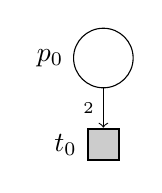
\begin{tikzpicture}

      % PLACES AND TRANSITIONS

      \node[place] (p0)  {};
      \node[transition, anchor=north] (t0) at ($(p0.south)-(0,.5)$) {};

      % LABELS

      \node[anchor=east] (tzLabel) at ($(t0.west)$) {$t_0$};
      \node[anchor=east] (pzLabel) at ($(p0.west)$) {$p_0$};
      
      % ARCS
      \draw[->] ($(p0.south)$) -- ($(t0.north)$) node[midway,left] {\ssmall $2$};
      
    \end{tikzpicture}
  };

  % PDI idp0
  
  \draw       
  node [dipchip, num pins=10, hide numbers,
  no topmark, external pins width=0]
  (idp0) at ($(pn.east)+(3.5,0)$) {};

  \node[anchor=south] at ($(idp0.north)$) {$\gamma(p_0)$};

  \draw ($(idp0.bpin 2)$)
  node [anchor=west, font=\ssmall]  {\tt oaw(i)}
  -- ++(-.3,0)
  node[anchor=east,font=\ssmall] {\tt 2};
  
  \draw ($(idp0.bpin 3)$)
  node [anchor=west, font=\ssmall] {\tt oat(i)}
  -- ++(-.3,0)
  node[anchor=east,font=\ssmall] {\tt basic};

  \draw ($(idp0.bpin 4)$)
  node [anchor=west, font=\ssmall]  {\tt otf(i)};

  \draw ($(idp0.bpin 9)$)
  node [anchor=east, font=\ssmall]  {\tt oav(i)};

  \draw ($(idp0.bpin 8)$)
  node [anchor=east, font=\ssmall]  {\tt rtt(i)};

  \draw ($(idp0.bpin 7)$)
  node [anchor=east, font=\ssmall]  {\tt pah(i)};
  
  % TDI idt0
  
  \draw       
  node [dipchip, num pins=10, hide numbers,
  no topmark, external pins width=0]
  (idt0) at ($(idp0.east)+(2,0)$) {};

  \draw ($(idt0.bpin 2)$)
  node [anchor=west, font=\ssmall]  {\tt iav(j)};

  \draw ($(idt0.bpin 3)$)
  node [anchor=west, font=\ssmall]  {\tt rt(j)};

  \draw ($(idt0.bpin 4)$)
  node [anchor=west, font=\ssmall]  {\tt pah(j)};

  \node[anchor=south] at ($(idt0.north)$) {$\gamma(t_0)$};

  \draw ($(idt0.east)$)
  node [anchor=east, font=\ssmall]  {\tt f};

  % INTERCONNECTIONS

  \draw[red,->-=.5] ($(idt0.south east)-(-.25,.4)$) -- ($(idp0.south west)-(.25,.4)$) node[red, midway, above] {\ssmall $id_{frd}$};
  \draw[red,->-=.5] ($(idt0.east)$) -| ($(idt0.south east)-(-.25,.4)$);
  \draw[red,->-=.5] ($(idp0.south west)-(.25,.4)$) |- ($(idp0.bpin 4)$);
  \draw[red,->-=.5] ($(idp0.bpin 9)$) -- ($(idt0.bpin 2)$) node[red, midway, above] {\ssmall $id_{av}$};
  \draw[red,->-=.5] ($(idp0.bpin 8)$) -- ($(idt0.bpin 3)$) node[red, midway, above] {\ssmall $id_{rt}$};
  \draw[red,->-=.5] ($(idp0.bpin 7)$) -- ($(idt0.bpin 4)$) node[red, midway, above] {\ssmall $id_{pah}$};
  
  % TRANSLATION ARROW
  
  \node at ($(pn.east)!.3!(idp0.west)$) {\Huge$\rightarrow$};

\end{circuitikz}


\end{document}
%%% Local Variables:
%%% mode: latex
%%% TeX-master: t
%%% End:
